\documentclass[10pt,twocolumn,letterpaper]{article}

\usepackage{acvs}
\usepackage{times}
\usepackage{epsfig}
\usepackage{graphicx}
\usepackage{amsmath}
\usepackage{amssymb}

% Include other packages here, before hyperref.
\usepackage{dsfont}

% If you comment hyperref and then uncomment it, you should delete
% egpaper.aux before re-running latex.  (Or just hit 'q' on the first latex
% run, let it finish, and you should be clear).
\usepackage[pagebackref=true,breaklinks=true,letterpaper=true,colorlinks,bookmarks=false]{hyperref}

\iccvfinalcopy % *** Uncomment this line for the final submission

\def\iccvPaperID{} % *** Enter the Paper ID here
\def\httilde{\mbox{\tt\raisebox{-.5ex}{\symbol{126}}}}

% Pages are numbered in submission mode, and unnumbered in camera-ready
\ificcvfinal\pagestyle{empty}\fi

\begin{document}

%%%%%%%%% TITLE - PLEASE UPDATE
\title{CoCa: Contrastive Captioners are Image-Text Foundation Models~\cite{coca} \\ {\rm {\normalsize Minji Kim (minji@snu.ac.kr; 2020-28702), Dept. of Electrical and Computer Engineering, Seoul National University}}}   % **** Enter the paper title and student information here

\maketitle
\thispagestyle{empty}

%%%%%%%%% BODY TEXT - ENTER YOUR RESPONSE BELOW

%%%%%%%%%%%%%%%%%
%%%%%%%%%%%%%%%%%
\section{Introduction}
Large-scale Vision-Language Pretraining (VLP) models is getting significant attention because of their scalability to downstream tasks.
This paper presents Contrastive Captioner (CoCa) to pretrain an image-text encoder-decoder foundation model with joint training with contrastive loss (like CLIP~\cite{clip}) and captioning loss (like SimVLM~\cite{simvlm}).
The pretrained CoCa can be applied to various downstream tasks including visual recognition, vision-language alignment, image captioning and multi-modal understanding with zero-shot transfer.
The overview of CoCa is illustrated in fig.~\ref{fig:overview}.



%%%%%%%%%%%%%%%%%
%%%%%%%%%%%%%%%%%
\section{Preliminaries}

Vision-language foundation models can be categorized into three:
(1) \textbf{Single-encoder models} are pretrained with cross-entropy loss on image classification datasets, \eg, ImageNet.
The image encoder provides generic \textit{visual representations} for various downstream tasks, but it regards image annotations as labeled vectors and cannot explore the free-form natural language labels.
(2) \textbf{Dual-encoder models} are pretrained with two parallel encoders with a contrastive loss on web-scale noisy image-text pairs.
These models enable the tasks to infer the \textit{cross-modal alignment} such as zero-shot image classification and image-text retrieval, but they are not directly applicable for joint vision-language understanding tasks, \eg, visual question answering (VQA), because joint multi-modal representation learning is not included in their pipelines.
(3) \textbf{encoder-decoder models} takes images on the encoder side and applies language modeling loss on the decoder outputs to attain text representations for \textit{multi-modal understanding} tasks.
However, these methods do not produce text-only representations that are aligned with image embeddings.

Unlike existing approaches, CoCa is a unified approach for single-encoder, dual-encoder, and encoder-decoder paradigms, and thus is applicable to more wide range of downstream tasks.



%%%%%%%%%%%%%%%%%
%%%%%%%%%%%%%%%%%
\section{Contrastive Captioner (CoCa)}

Similar to general image-text encode-decoder models, CoCa encodes images to latent embeddings through a neural network encoder such as ViT or ConvNets, followed by decoding texts with standard Transformer decoders.
The difference with existing decoder is that CoCa removes cross-attention in the first half of the decoder layers for processing unimodal text representations, while the last half cross-attends to the image encoder for multi-modal representations.
Detailed illustrations can be found in Fig.~\ref{fig:detail}.






%%%%%%%%%%%%%%%%%
%%%%%%%%%%%%%%%%%
\section{Some Interesting Parts in Experiments}

CoCa is also applied to video recognition task in the experimental section.
Multiple frames of videos are fed into the shared image encoder individually, and the additional pooler is trained on top of the spatial and temporal feature tokens.
As can be seen in the right table of Fig.~\ref{fig:experiment},
CoCa achieves better performance than a video-based Transformer such as ViViT~\cite{vivit} even without video-level representation learning.


\begin{figure}[t]
    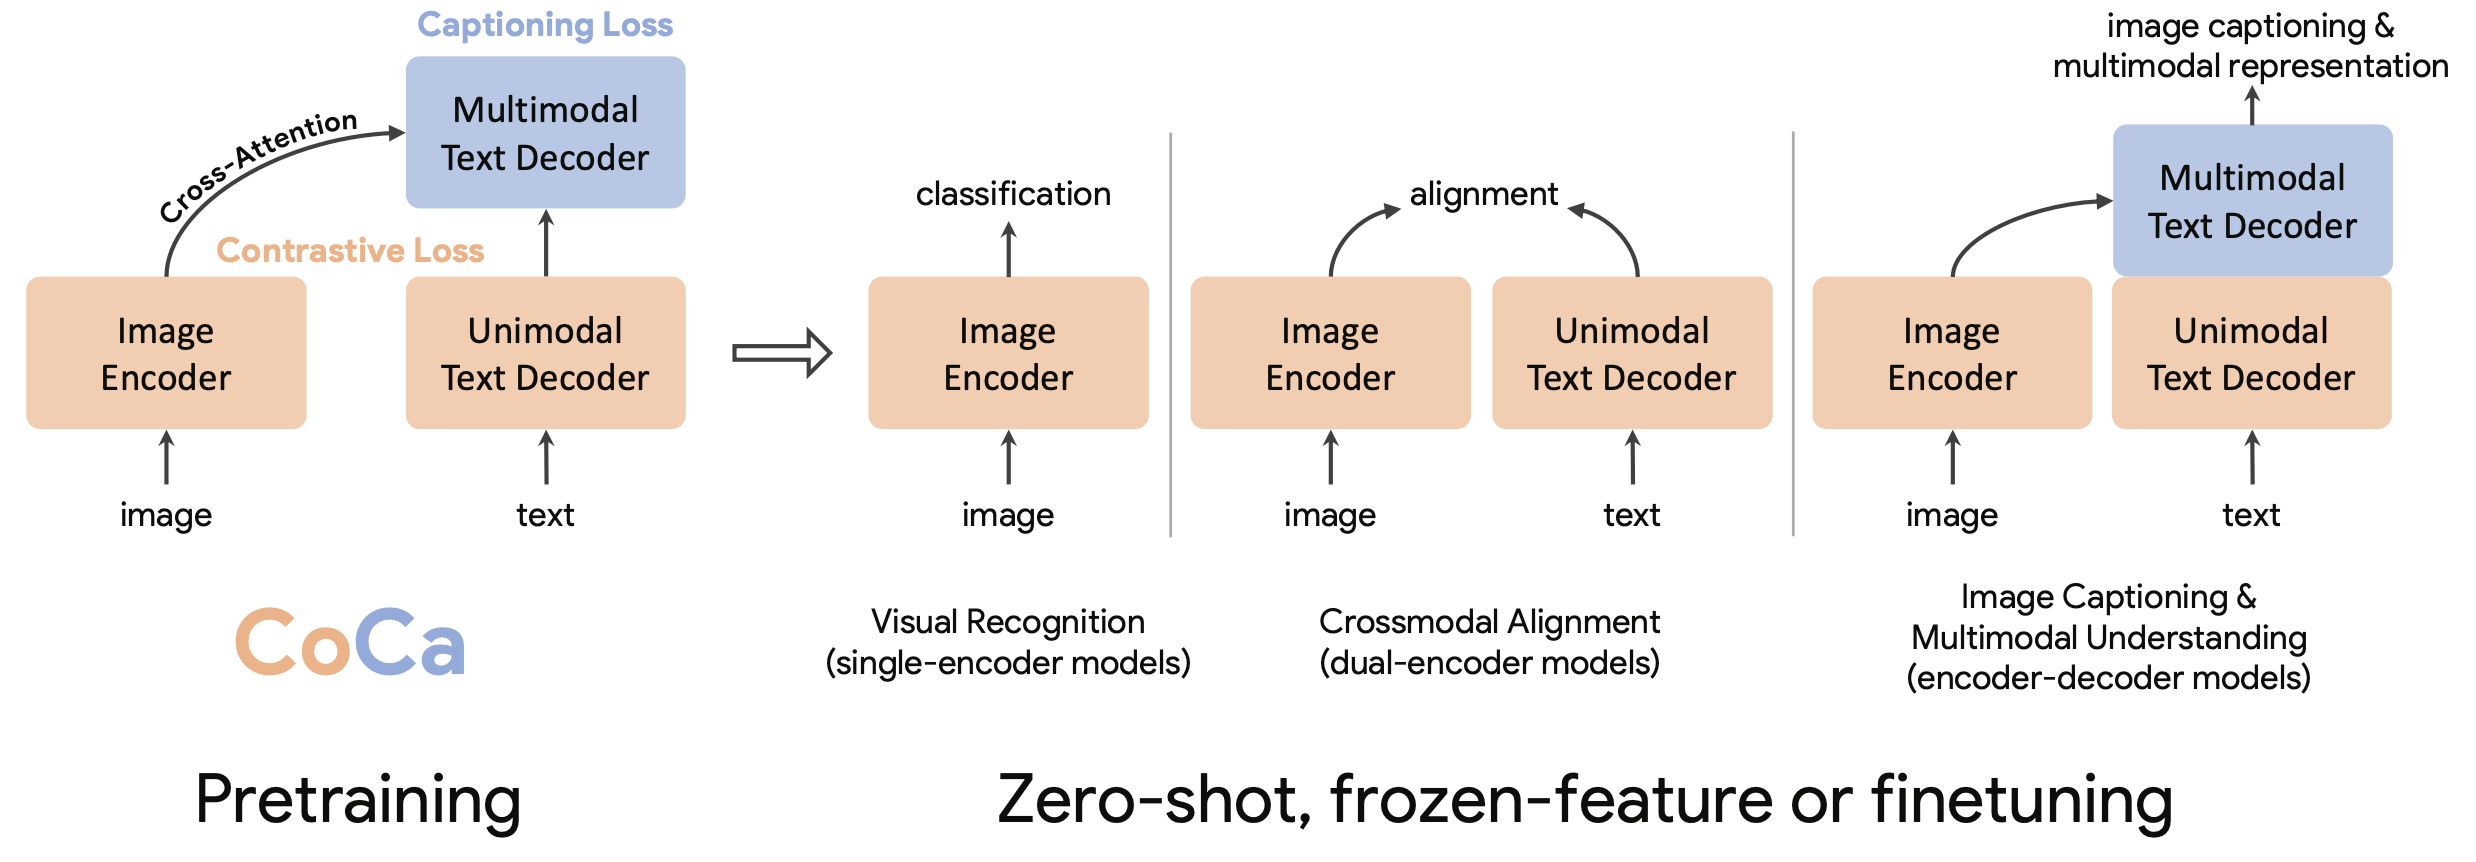
\includegraphics[width=\linewidth]{assets/coca_overview.png}
    \caption{\label{fig:overview}Overview of CoCa.}
\end{figure}

\begin{figure}[t]
    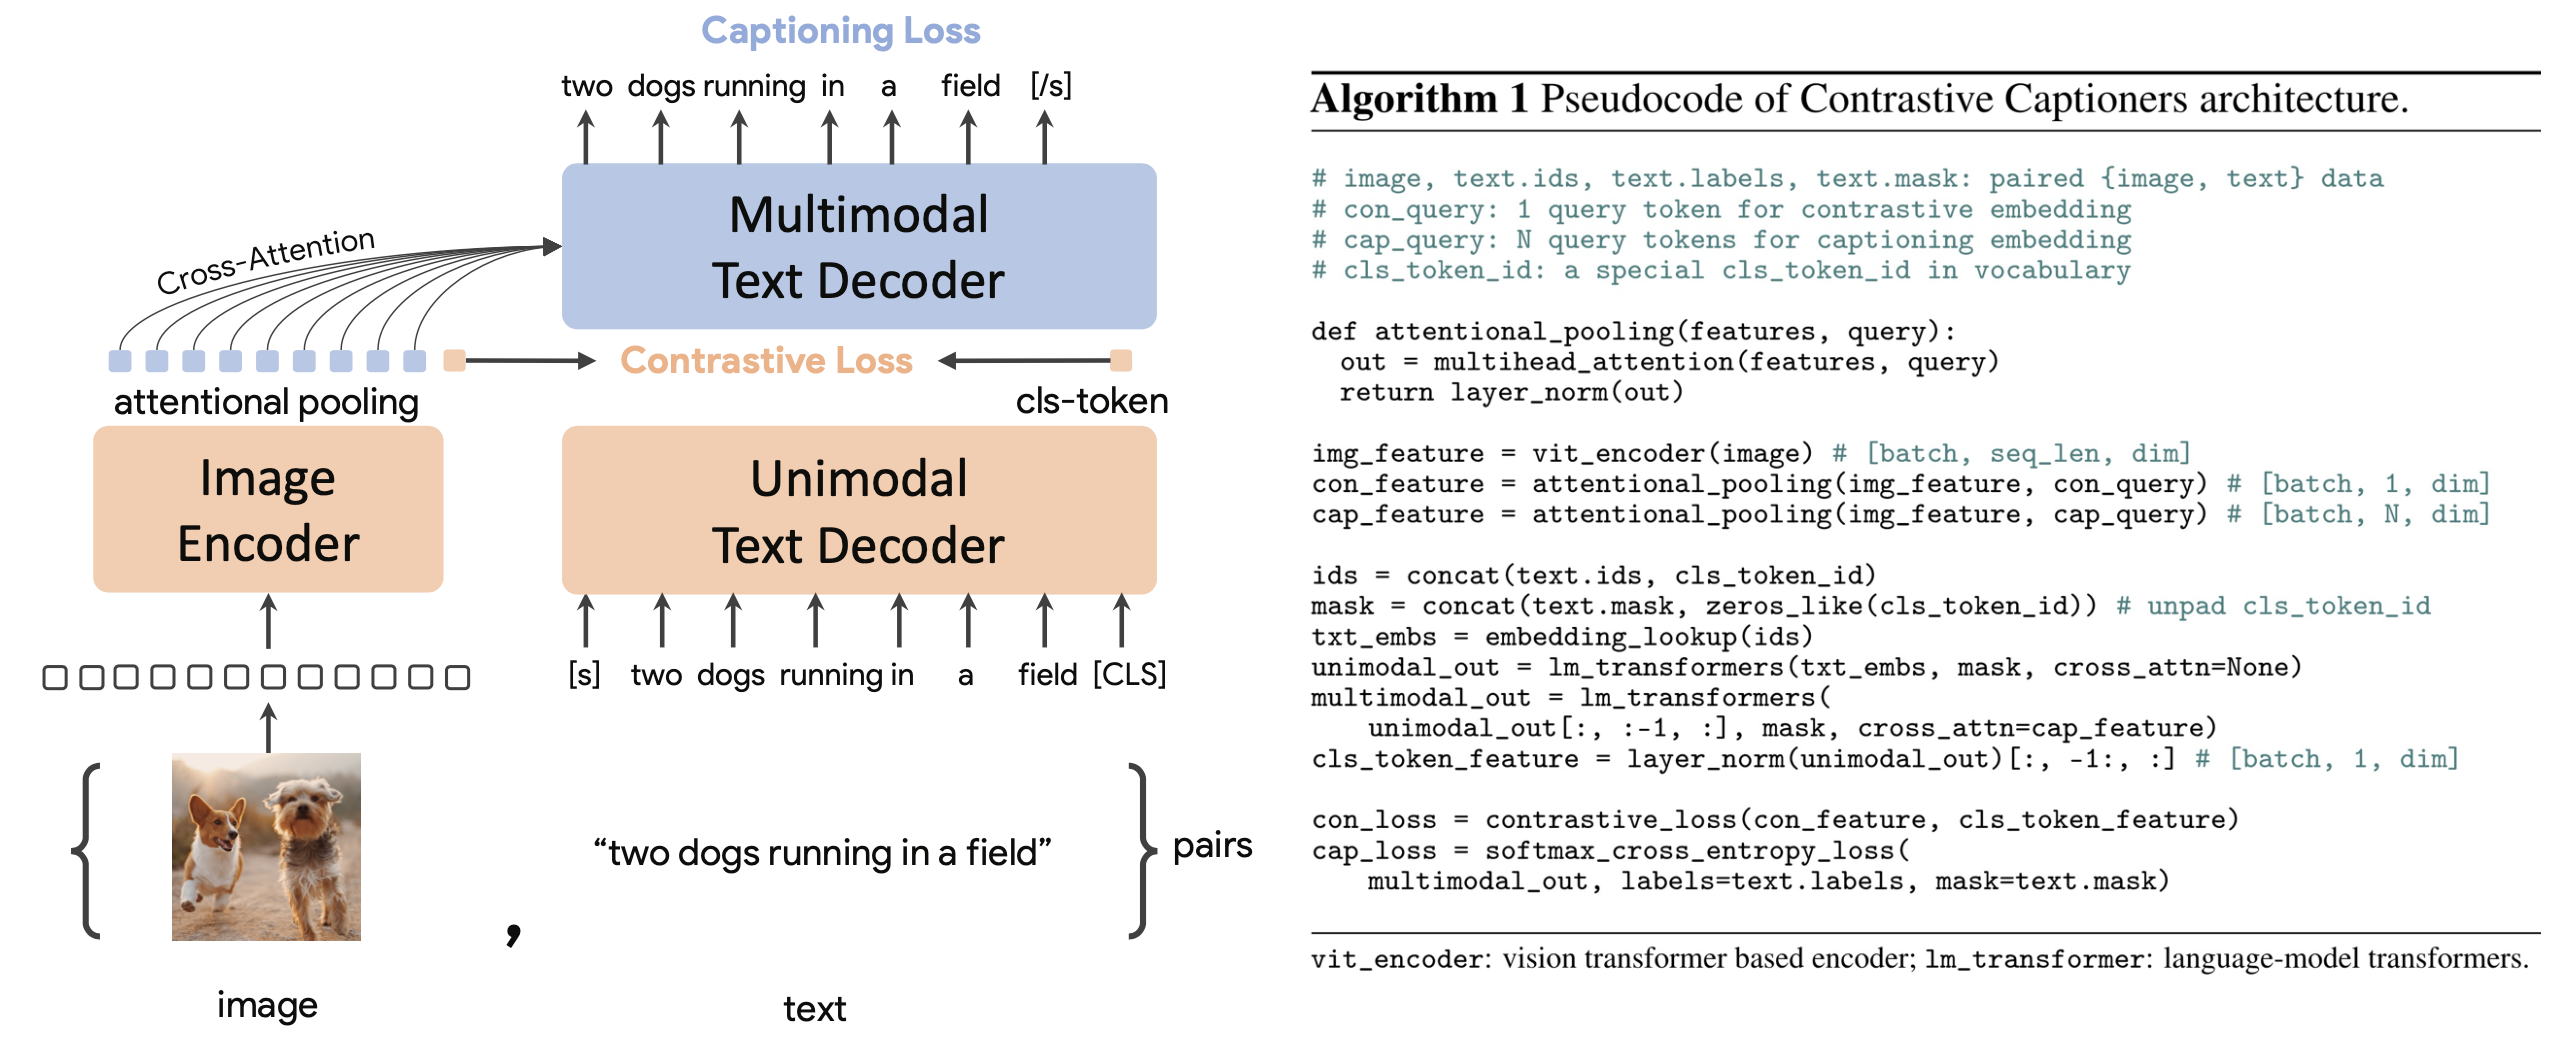
\includegraphics[width=\linewidth]{assets/coca_detail.png}
    \caption{\label{fig:detail}Detailed illustration and pseudo code of CoCa.}
\end{figure}

\begin{figure}[t]
    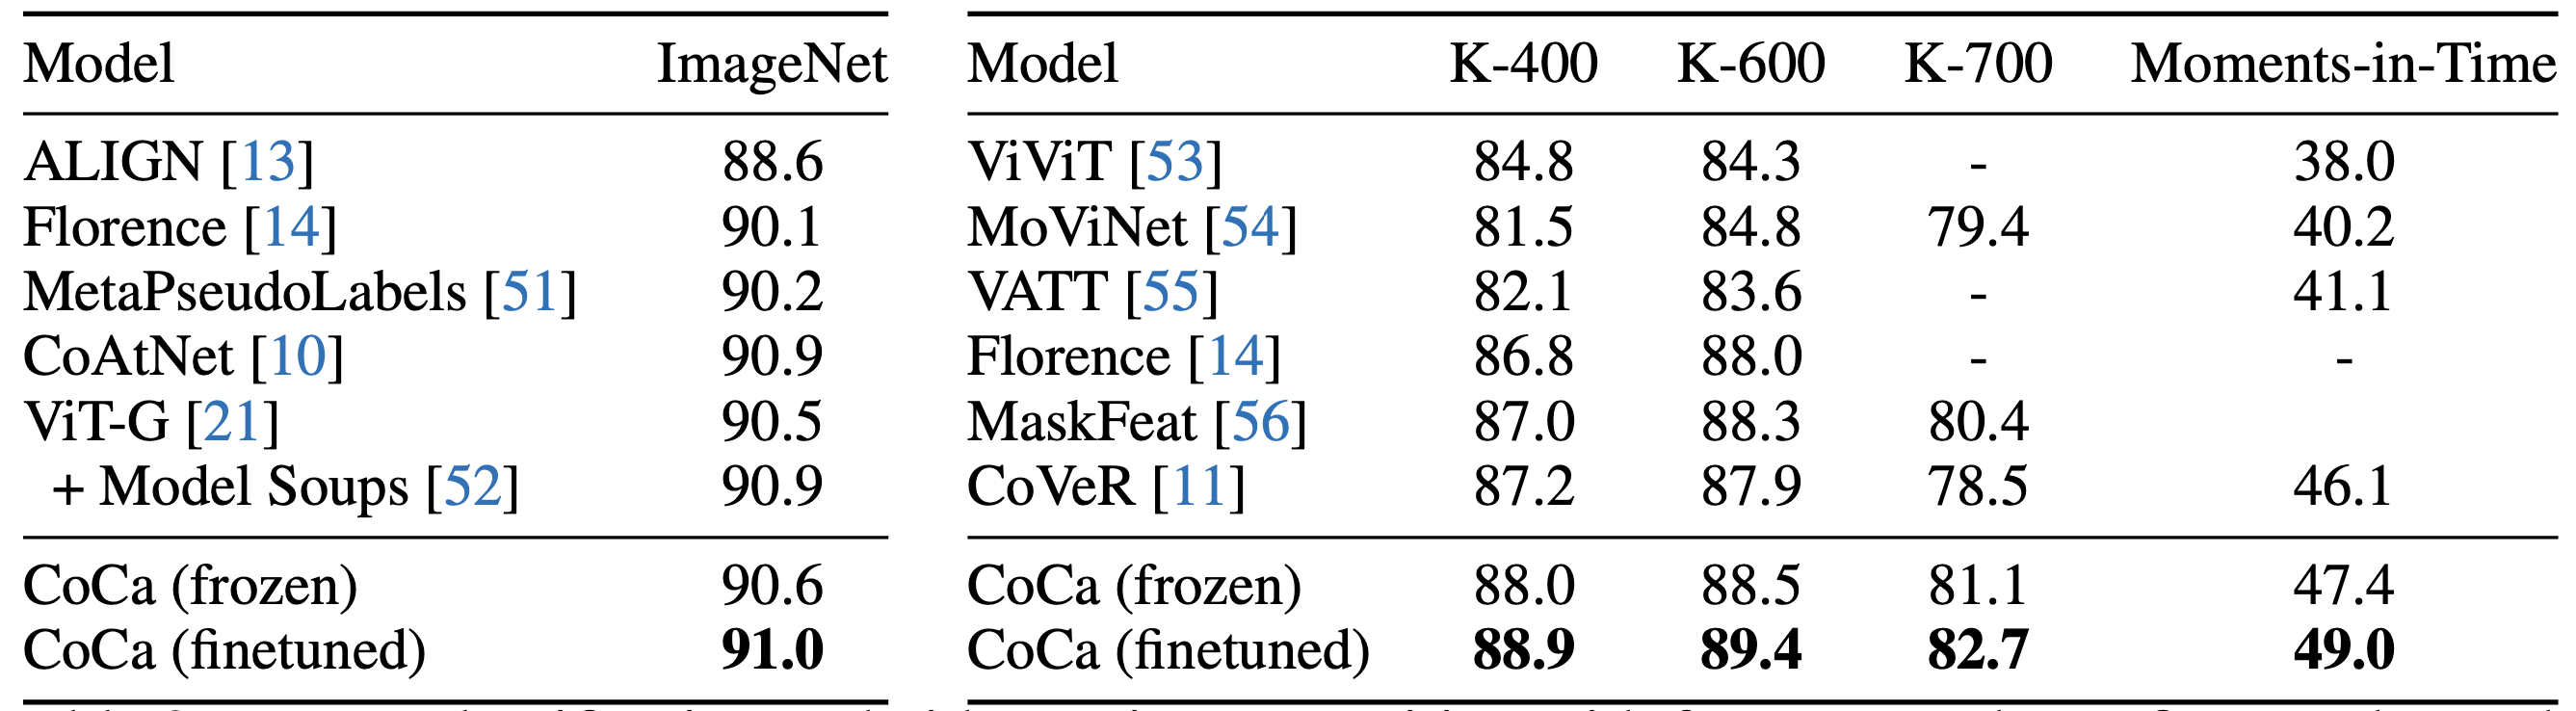
\includegraphics[width=\linewidth]{assets/experiment.png}
    \caption{\label{fig:experiment}Experimental results on image classification and video action recognition tasks.}
\end{figure}



{\small
\bibliographystyle{ieee}
\bibliography{egbib}
}

\end{document}
